\chapter{引言}
\label{chap:introduction}

\section{什么是机器学习}
\label{sec:what-is-machine-learning}

\subsection{什么是学习}

儿童看过一些猫和狗以后，往往能认出一只从未见过的猫；学生练习解方程，也希望掌握的
方法能用于新题。我们把这些变化称为“学习”，关心的不只是记住了哪些例子，还包括这些
经验怎样改变了以后处理问题的能力。驾驶员根据路况和反馈改进操作，同样如此。
一次疲劳造成的失误或短暂的兴奋也会改变当下表现，但谈论学习时，我们更关心由经验
带来的、能够保持一段时间的变化。

这就留下了一个更具体的问题：计算机程序怎样利用有限经验形成处理新输入的规则，又该怎样
检验这种能力？本章通过一个垃圾邮件分类案例回答这两个问题。沿着建模、训练、预测与评价
的过程，我们将逐步认识任务、经验和性能度量，并区分“在已有样本上做得好”与“能够处理
新样本”。机器学习理论部分将进一步研究，在明确的数据、损失和比较条件下，能否证明算法
用有限经验得到符合标准的结果，也就是这个学习问题是否可学习。即使这项结论成立，模型在
真实流程中能否适应人群、环境、权限和风险要求，仍需由机器学习可信性部分另行检验。

哲学很早就在追问经验如何支持知识。\term{演绎}（deduction）从给定前提出发，推出由前提
保证的结论；\term{归纳}（induction）则试图从有限的观察形成超出这些观察的一般判断。
D.~Hume（休谟）指出，过去经验本身并不能以演绎方式保证未来仍与过去相似
\scite{hume1748}。机器学习同样面对这个问题：训练数据永远只是已经见过的有限情形，
系统却被要求处理尚未见过的输入。机器学习系统要作出这种判断，必然还依赖关于哪些规律
值得延伸到新情形的假设。

要研究这种变化，还需要决定观察什么。心理学既研究可见的行为变化，也研究经验如何改变
内部知识与表征，即学习者组织和理解信息的方式。\term{条件作用}（conditioning）关注
刺激、反应和结果之间逐渐形成的联系，例如某种行为得到奖励后，发生频率可能增加；
认知取向则进一步讨论记忆、概念和策略如何改变。不同定义强调的对象并不相同，因此
不能把学习简单等同于“记住更多事实”。
一种有影响的功能性定义把学习理解为环境中的规律所引起的行为改变\scite{dehouwer2013}。

\subsection{从学习到机器学习}
\term{机器学习}（machine learning, ML）借用了“从经验中改变”的核心直觉，但机器没有必要复制人的心理过程。
对计算机程序而言，更直接的问题是：如果逐条编写规则过于困难，能否让程序利用已有
数据或交互反馈，自动形成一套在新输入上也有效的处理方法？例如，垃圾邮件的写法不断
变化，维护一张完整的关键词和例外规则清单很快就会变得困难；历史邮件却提供了大量
可以利用的经验。

这一设想由多条研究路线逐渐汇合。McCulloch和Pitts用理想化神经元组成网络，
Turing提出通过教育和经验改变机器，Rosenblatt的感知机让分类错误直接调整连接权重，
Samuel的跳棋程序则利用已有棋局和自我对弈改进决策
\scite{mcculloch1943,turing1950,rosenblatt1958,samuel1959}。这些工作已经呈现出
后来监督学习与交互学习的不同经验形式。

有了能按样本调整的程序，还需要回答它为何适用于新样本，以及怎样训练更复杂的模型。
Vapnik和Chervonenkis等人的工作把有限样本与候选规则复杂度联系起来
\scite{vapnik1971}；\term{误差反向传播}（error backpropagation）提供了调整多层网络参数的计算方法
\scite{rumelhart1986}；更大规模的数据、计算与模型又推动了\term{表示学习}
（representation learning）和\term{深度学习}（deep learning），使模型
能够从复杂输入中形成任务所需的表示\scite{lecun2015}。这些路线分别推进统计保证、
优化方法和表示能力，共同服务于“怎样把有限经验转化为处理新情形的能力”。

机器学习与\term{人工智能}（artificial intelligence）、\term{统计学}（statistics）、
\term{概率论}（probability theory）、\term{优化}（optimization）、信息论、信号处理、
控制和数据系统都有交叉。\term{数据挖掘}（data mining）与机器学习共享分类、聚类和
\term{异常检测}（anomaly detection）等方法，但更强调从已有数据发现可用模式。
人工智能提供任务与行动框架，概率论与统计学描述不确定性和估计，优化研究求解方法，
信息论与信号处理提供编码、表示和变换工具，控制关注行动与反馈，数据系统提供采集、存储
和计算基础；应用领域还决定标签、错误代价与使用约束。机器学习因此不是单纯“选一个模型”，
而是要把任务、经验、模型、训练过程和评价方式共同规定清楚。下面的定义先把其中三个最基本
的要素固定下来。

\subsection{机器学习的定义}

这些研究路线都谈到“从经验中改进”，但要判断一个程序是否真的学到了东西，还必须说明
它在做什么、用什么衡量改进，以及利用了哪些经验。T.~M.~Mitchell的经典定义把这三点
明确联系起来\scite{mitchell1997}。

\begin{definition}[机器学习]
\label{def:machine-learning}
对于某类任务 $T$ 和性能度量 $P$，如果一个计算机程序在任务 $T$ 上按 $P$ 衡量的性能
因经验 $E$ 而有所改善，就称该程序从经验 $E$ 中进行了学习。
\end{definition}

定义~\ref{def:machine-learning}中的三个要素各有具体含义：

\begin{itemize}
  \item \term{任务}（task, $T$）说明希望系统完成什么，例如判断邮件是否为垃圾邮件；
  \item \term{性能度量}（performance measure, $P$）说明怎样判断任务完成得好不好，
    例如分类正确的比例或漏放垃圾邮件的数量；
  \item \term{经验}（experience, $E$）说明系统从什么信息中学习，例如带人工标签的
    历史邮件，也可以是没有标签的数据、用户反馈或与环境交互得到的奖励。
\end{itemize}

三个要素必须放在一起理解。同一批邮件可以支持垃圾邮件分类，也可以用于发现邮件主题；
同一个分类器按准确率衡量可能表现良好，按误拦正常邮件的代价衡量却未必合格。
“因经验$E$而有所改善”也不意味着每增加一个样本，指标都要单调上升。经验$E$可以是一批
已标注样本、交互记录或其他反馈；定义要求用$P$检验这些经验是否改善了任务表现，而不是
把$E$解释成必须逐步增加的样本数量。

\section{例子：垃圾邮件分类}
\label{sec:spam-classification-example}

回到垃圾邮件的问题。逐条维护拦截规则很难覆盖不断变化的写法，我们希望利用已经判定
类别的历史邮件，学出一套处理新邮件的规则。本节沿着数据准备、建模、训练、预测和评估
展开这个过程。邮件和标签均为教学构造。完整数据与训练配置保存在随书脚本
\code{introduction-spam-example.py}中，逐次损失记录见同目录的
\code{introduction-training-loss.csv}；这些计算结果不代表真实邮件系统的效果。

我们希望根据一封邮件中可用的信息，将它判为垃圾邮件或正常邮件。这是一个
\term{二分类}（binary classification）问题，即从两个候选类别中选择一个。
用\term{标签}（label）记录每封邮件的已知类别：约定垃圾邮件是\term{正类}（positive class），
标签为$1$；正常邮件是\term{负类}（negative class），标签为$0$。正负只是计数和计算时的约定，
不表示类别的好坏。
表~\ref{tab:spam-three-elements}把三个要素落实到这个问题中。

\begin{table}[htbp]
  \centering
  \small
  \begin{tabularx}{\linewidth}{@{}lX@{}}
    \toprule
    \textbf{要素} & \textbf{在垃圾邮件分类中的含义} \\
    \midrule
    任务 $T$ & 输入一封邮件，输出“垃圾邮件”或“正常邮件”。 \\
    性能度量 $P$ & 考察测试邮件中分类正确的比例，并分别记录误拦正常邮件和漏放垃圾邮件。 \\
    经验 $E$ & 历史邮件、由人工给出的类别标签，以及据此形成的训练反馈。 \\
    \bottomrule
  \end{tabularx}
  \caption{垃圾邮件分类问题的任务、性能度量与经验。三个要素共同规定了“学得更好”的含义。}
  \label{tab:spam-three-elements}
\end{table}

评价学习结果需要参照物。\term{基线}（baseline）就是用来比较的简单方案；本例把所有邮件
都判为训练集中较多的类别，也就是正常邮件。
如果测试集中大多数邮件是正常邮件，这个办法即使完全没有识别垃圾邮件，也可能得到不低的
准确率。因此，后面既要与基线比较，也要分别检查两类错误。

\subsection{从邮件到样本与特征}

计算机需要从邮件中读取具体信息，才能作出“是否可疑”的判断。我们把原始邮件转换成模型
可以处理的\term{表示}（representation），也就是约定用哪些量描述它。
这些量称为\term{特征}（feature）。可用信息包括发件人及其域名、主题和
正文中的词语、字符组合、链接与附件、邮件头、发送时间以及用户过去是否与发件人通信。
现实系统通常需要综合多类信息，也不能预先认定某一个特征在所有环境中都可靠。

为了让单封邮件的预测和后续评价能够手工复核，本例只用两个计数特征作为模型输入。
教学数据中，相同或相近的计数也可能对应不同标签，因此这两个特征提供的是有限的分类线索，
而不是决定标签的规则。令$x_1$为正文中促销提示词出现的次数，$x_2$为外部链接的数量，一封邮件
便表示为特征向量$\bm{x}=(x_1,x_2)^{\top}\in\mathbb{R}^{2}$。这个简化只服务于教学案例；它省略了
发件人身份、上下文和附件内容等信息，不能据此推断真实垃圾邮件只由这两个特征决定。

在这个带标签的案例中，一封邮件的特征与标签组成一个\term{样本}（sample）
$(\bm{x}_i,y_i)$，即一次可供学习的记录；下标$i$标识第$i$封邮件。多个样本组成
\term{数据集}（dataset）。
表~\ref{tab:spam-data-excerpt}展示了数据的一部分。原始文本和特征向量是不同层次的对象：
前者是现实中收集的信息，后者是为当前模型构造的输入。

\begin{table}[t]
  \centering
  \footnotesize
  \begin{tabularx}{\linewidth}{@{}llXcccl@{}}
    \toprule
    \textbf{编号} & \textbf{子集} & \textbf{邮件片段} & $x_1$ & $x_2$ & $y$ & \textbf{类别} \\
    \midrule
    \code{tr01} & 训练 & “限时优惠，立即领取……” & 3 & 2 & 1 & 垃圾邮件 \\
    \code{tr06} & 训练 & “周会改至下午三点” & 0 & 0 & 0 & 正常邮件 \\
    \code{tr11} & 训练 & “优惠券报销说明” & 2 & 0 & 0 & 正常邮件 \\
    \code{va02} & 验证 & “会员权益，详情见链接” & 1 & 2 & 1 & 垃圾邮件 \\
    \code{va03} & 验证 & “本周三场促销培训” & 3 & 0 & 0 & 正常邮件 \\
    \code{te02} & 测试 & “两项优惠，见附件链接” & 2 & 1 & 0 & 正常邮件 \\
    \code{te07} & 测试 & “专属优惠今日有效” & 2 & 0 & 1 & 垃圾邮件 \\
    \code{te08} & 测试 & “优惠详情见两个链接” & 1 & 2 & 0 & 正常邮件 \\
    \bottomrule
  \end{tabularx}
  \caption{教学数据的部分样本。$x_1$为促销提示词次数，$x_2$为外部链接数，
  标签 $y=1$ 表示垃圾邮件。训练集、验证集和测试集承担不同职责。}
  \label{tab:spam-data-excerpt}
\end{table}

如果反复用同一批邮件学习、挑选方案和报告成绩，就难以判断模型能否处理真正的新邮件。
为此，在开始训练前，把历史数据划分为\term{训练集}（training set）、
\term{验证集}（validation set）和\term{测试集}（test set）：分别用来学习参数、选择训练
轮数等配置，以及在选择完成后评价结果。表中的“子集”一列记录了这项分工。
需要从数据估计的预处理规则也只用训练集确定，例如根据词频选择词表，或计算用于调整
特征尺度的均值。否则，后面的评价已经提前利用了本应保留的信息。

\subsection{对问题进行建模}

要从有限的邮件样本得到可用于新邮件的分类器，必须先对特征与结果之间的关系作出假设。
这里假设垃圾邮件倾向可以由两个特征的线性组合描述：促销提示词或链接数量每增加一个单位，
都会使得分改变一个由相应权重决定的量。得分没有固定的取值范围，不能直接当作概率。
为了赋予输出概率语义，记随机特征向量为$\bm{X}$，其取值在$\mathbb{R}^2$中；随机标签为
$Y$，其取值在$\{0,1\}$中；$\bm{x}$表示一封邮件的特征实现。把模型参数记为
$\bm{\theta}=(b,w_1,w_2)^{\top}\in\Theta$，本例取$\Theta=\mathbb{R}^3$。进一步约定
$Y\mid\bm{X}=\bm{x}\sim\operatorname{Bernoulli}(p_{\bm{\theta}}(\bm{x}))$：给定邮件特征后，
标签为1的概率是$p_{\bm{\theta}}(\bm{x})$，标签为0的概率是$1-p_{\bm{\theta}}(\bm{x})$。
本例用\term{逻辑函数}（logistic function）把线性得分映射到$(0,1)$：得分越大，
输出越接近1；得分越小，输出越接近0。这个计算关系写为
\begin{align}
  z_i &= b+w_1x_{i,1}+w_2x_{i,2}, \\
  p_{\bm{\theta}}(\bm{x}_i)
  =f_{\bm{\theta}}(\bm{x}_i)
  =\hat{p}_i
  &=\sigma(z_i)=\frac{1}{1+\exp(-z_i)}.
  \label{eq:spam-model}
\end{align}
这个分类\term{模型}（model）规定输入怎样产生输出。在上述Bernoulli条件模型约定下，
$\hat{p}_i$才被解释为模型对“第$i$封邮件是垃圾邮件”的概率估计；仅仅把任意得分压到
$(0,1)$内，并不足以自动获得概率含义。
式中的$\exp(-z_i)=e^{-z_i}$是指数函数；$\sigma$是逻辑函数的简写。
概率还需要转换成类别：当$\hat{p}_i\geq 0.5$时预测$\hat{y}_i=1$，否则预测$\hat{y}_i=0$。
这里预先选取$0.5$作为分类\term{阈值}（threshold），决定多大的垃圾邮件概率会触发拦截。
它便于演示，但不表示在误拦与漏放成本不对称时仍然最优。

$b$是\term{偏置}（bias），决定两个特征都为零时的得分；$w_1,w_2$是特征的
\term{权重}（weight），分别决定多一个促销词或外部链接会使得分改变多少。
这些需要从数据中确定的量称为\term{模型参数}（model parameters）。每一组
$\bm{\theta}\in\Theta$都确定一条具体的分类规则，所有允许参数产生的函数关系
$\mathcal H=\{f_{\bm{\theta}}:\bm{\theta}\in\Theta\}$共同组成\term{假设空间}
（hypothesis space）。选择式~\eqref{eq:spam-model}这样的
函数形式，与在训练中确定某个具体的$\bm{\theta}$，是两个不同决定：前者规定可以考虑哪些
模型，后者从中选出一个具体模型。

有限样本通常不能唯一决定对所有新邮件的预测。即使训练算法在预先限定的逻辑模型中选出
唯一参数，这种唯一性也依赖模型形式、损失和选择规则；有限数据本身并未排除其他规律。
例如，一条规则只看两个计数，另一条还查看发件人；二者可以在已见邮件上作出相同判断，
却对一封未见邮件给出不同预测。我们先对两个计数特征线性加权得到得分，再用逻辑函数和
固定阈值确定分类，这些预先作出的选择构成\term{归纳偏置}
（inductive bias）。归纳偏置让学习算法优先考虑某一类规律，使从有限经验推广到未见样本
成为可能，同时也限制了模型能表达的关系。本例只保留两个计数；即使两封邮件的语境
完全不同，只要计数相同，模型就会给出相同预测。若区分它们需要发件人或上下文信息，
调整权重也无法补回输入中已经丢失的内容。

有了候选的分类规则，还需要比较哪一组参数预测得更好。\term{损失函数}（loss function）
给一次预测的错误程度计分，损失越小，表示这次预测越符合目标。本例输出的是概率，
因此采用\term{二分类交叉熵}（binary cross-entropy）：它检查模型给真实类别分配了多少
概率，分配得越少，惩罚越大。对于标签$y_i\in\{0,1\}$，损失写为
\begin{equation}
  \ell(\hat{p}_i,y_i)
  =-y_i\log\hat{p}_i-(1-y_i)\log(1-\hat{p}_i).
  \label{eq:binary-cross-entropy}
\end{equation}
这里$\log$取自然对数。以一封真正的垃圾邮件为例，它的标签为$y_i=1$，损失为$-\log\hat{p}_i$。
如果模型预测它是垃圾邮件的概率为 $0.9$，损失约为 $0.105$；如果预测概率只有 $0.1$，
损失则约为 $2.303$。因此，模型为邮件的真实类别分配的概率越高，损失越小；概率越低，
损失越大。

只比较一封邮件不足以选择参数。若训练集包含$n$个样本，我们把各次预测的损失取平均，
得到\term{经验风险}（empirical risk），用它概括模型在整批训练邮件上的错误代价：
\begin{equation}
  \hat{R}_{\mathrm{train}}(\bm{\theta})
  =\frac{1}{n}\sum_{i=1}^{n}\ell\bigl(f_{\bm{\theta}}(\bm{x}_i),y_i\bigr).
  \label{eq:spam-empirical-risk}
\end{equation}
在允许的参数中寻找平均训练损失最小的一组，称为\term{经验风险最小化}
（empirical risk minimization, ERM）。如果最小值能够取到，这个目标可以写为
\begin{equation}
  \hat{\bm{\theta}}
  \in\argmin_{\bm{\theta}\in\Theta}\hat{R}_{\mathrm{train}}(\bm{\theta}).
  \label{eq:spam-erm}
\end{equation}
这里的$\argmin$表示使目标函数达到最小值的参数集合；实际训练往往只是在有限计算内
寻找较好的近似解。损失函数服务于参数学习，性能度量服务于任务评估，二者可以一样，
也可以不同。本例用交叉熵来训练模型，
但最终对整个任务的结果进行评估还要看在测试数据上的准确率、误拦数和漏放数等指标。

\subsection{根据历史邮件进行训练}

目标已经写出，但计算机仍需要知道怎样调整参数。\term{训练}（training）就是利用训练
数据确定参数的过程。本例采用\term{梯度下降}（gradient descent）：在当前参数附近，
沿着损失下降的方向走一小步，然后重新计算并继续调整。从
$\bm{\theta}^{(0)}=(0,0,0)^{\top}$开始，更新规则为
\begin{equation}
  \bm{\theta}^{(t+1)}
  =\bm{\theta}^{(t)}-\eta\nabla_{\bm{\theta}}
  \hat{R}_{\mathrm{train}}\bigl(\bm{\theta}^{(t)}\bigr).
  \label{eq:spam-gradient-update}
\end{equation}
上标$(t)$表示第$t$次更新后的参数；$\nabla_{\bm{\theta}}$表示对参数求梯度。
梯度指向损失在当前位置增长最快的方向，所以更新时沿它的反方向移动。
\term{学习率}（learning rate）$\eta$控制每一步的幅度，本例取$\eta=0.35$。
本例的损失函数具有连续的导数，沿非零梯度的反方向走足够小的一步会使损失下降；
步子过大则未必如此。

权重和偏置由式~\eqref{eq:spam-gradient-update}更新，学习率和迭代次数却需要另外选择。
这类控制模型或学习过程的配置称为\term{超参数}（hyperparameter）。分类阈值也要事先
约定或通过验证集选择，不过在本例中，它只影响概率怎样变成类别，不参与交叉熵的参数更新。
本例在训练前固定阈值为$0.5$，并把$C=\{20,40,60\}$作为候选迭代次数集合；每个候选
都按验证准确率比较，若准确率相同，就选择迭代次数较小的候选。

\begin{algorithm}[垃圾邮件分类器的训练]
  \label{alg:spam-training}
  \begin{algorithmic}[1]
    \Require 训练集 $D_{\mathrm{train}}$，验证集 $D_{\mathrm{val}}$，
      学习率 $\eta$，候选迭代次数集合 $C=\{20,40,60\}$，分类阈值 $0.5$
    \Ensure 选定参数 $\hat{\bm{\theta}}$
    \State 初始化 $\bm{\theta}^{(0)}$
    \For{$t=0,\ldots,\max(C)-1$}
      \State 在训练集上计算经验风险及其梯度
      \State 按式~\eqref{eq:spam-gradient-update}得到 $\bm{\theta}^{(t+1)}$
      \If{$t+1\in C$}
        \State 按阈值 $0.5$ 在验证集上记录准确率
      \EndIf
    \EndFor
    \State 从验证准确率最高的候选中选取迭代次数最小者，记为 $\hat{\bm{\theta}}$
    \State \Return $\hat{\bm{\theta}}$
  \end{algorithmic}
\end{algorithm}

第一次更新把三个参数从零改为约$(-0.029,0.102,0.058)^{\top}$，平均训练损失随之从
$0.693$降至$0.658$。这说明更新改善了训练集上的预测，但还没有回答应当训练多久。
在20、40和60次参数更新这三个候选时点，每到一个时点，就保存当时的三个参数，并用它们对
验证集中的6封邮件进行分类。这样得到的是同一种模型在三个训练阶段的版本。验证集中的邮件
不参与参数更新，只用于比较这些版本的分类效果。

完成20次和40次参数更新后，模型都正确分类了6封验证邮件中的5封，准确率均为 $5/6$；
完成60次更新后，模型只正确分类了4封，准确率为 $4/6$。按照上述平局规则，最终采用
第20次更新后保存的参数，而不是训练
结束时的最后一组参数。选定参数为
\begin{equation}
  \hat{\bm{\theta}}=(-1.000,\,0.692,\,0.230)^{\top}.
  \label{eq:spam-fitted-parameters}
\end{equation}

\begin{table}[htbp]
  \centering
  \small
  \begin{tabularx}{\linewidth}{@{}rXXXX@{}}
    \toprule
    $t$ & $b^{(t)}$ & $w_1^{(t)}$ & $w_2^{(t)}$ & 训练损失 \\
    \midrule
    0  & $0.000$  & $0.000$ & $0.000$ & $0.693$ \\
    1  & $-0.029$ & $0.102$ & $0.058$ & $0.658$ \\
    20 & $-1.000$ & $0.692$ & $0.230$ & $0.452$ \\
    \bottomrule
  \end{tabularx}
  \caption{训练过程中参数与平均训练损失的变化。第20次迭代是验证集选定的检查点；
  表中数值由完整计算结果舍入得到。}
  \label{tab:spam-training-record}
\end{table}

图~\ref{fig:spam-training-loss}显示，继续训练仍会降低训练集损失，验证集交叉熵也缓慢下降，
但按$0.5$阈值计算的验证准确率并不因此持续提高。这说明，优化的损失与最终关心的
性能度量有关联，却不是同一个量。

\begin{figure}[htbp]
  \centering
  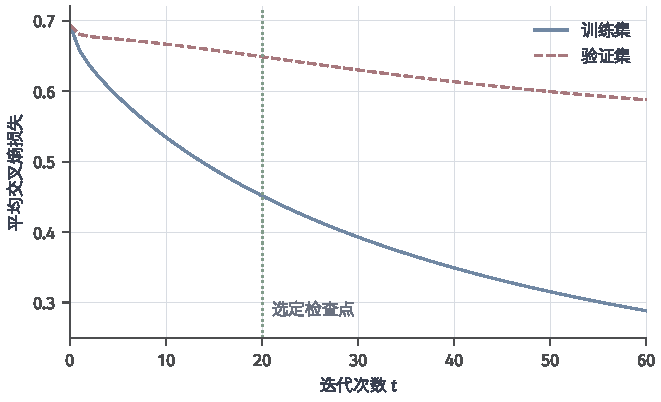
\includegraphics[width=\linewidth]{figures/02-foundations/01-basics/matplotlib/introduction-training-loss/figure.pdf}
  \caption{训练集和验证集上的平均交叉熵损失。蓝色实线表示训练曲线，红色虚线表示验证曲线，
  绿色竖线标出按验证准确率选定的第20次迭代；模型选择并非直接读取训练损失的最低点。}
  \label{fig:spam-training-loss}
\end{figure}

回看这次训练，模型形式、学习算法和训练结果承担了不同工作。
式~\eqref{eq:spam-model}规定特征怎样转换为概率，尚未给定其中的参数；
\term{学习算法}（learning algorithm）则规定怎样利用数据确定参数。本例的算法包括
梯度更新和验证选择两个环节，具体过程见算法~\ref{alg:spam-training}。
把选出的参数代入模型形式，才得到可以直接预测的具体函数。此后每收到一封新邮件，
只需计算这个函数，无须重做训练。

\subsection{对新邮件进行预测}

参数选定后，就可以处理新的输入了。使用学到的模型计算输出，称为\term{推理}
（inference）。本例的推理依次计算垃圾邮件概率和预测类别，不需要把真实标签作为输入，
也不更新模型参数。它既可以用于尚无标签的新邮件，也可以用于已有标签的测试邮件；
后一种情况只是让我们能在预测之后检查答案。

对于编号为
\code{new01}的新邮件，其特征为 $\bm{x}=(2,2)^{\top}$，代入选定参数得到
\begin{align}
  z&=-1.000+0.692\times 2+0.230\times 2=0.844,\\
  \hat{p}&=\sigma(0.844)=0.699.
\end{align}
因为 $0.699\geq 0.5$，模型把它预测为垃圾邮件。表~\ref{tab:spam-inference-results}
列出三个新样本的结果。

\begin{table}[htbp]
  \centering
  \small
  \begin{tabularx}{\linewidth}{@{}lXcccl@{}}
    \toprule
    \textbf{编号} & \textbf{邮件片段} & $(x_1,x_2)$ & $\hat{p}$ & \textbf{阈值} & \textbf{预测} \\
    \midrule
    \code{new01} & “会员优惠，点击两个链接” & $(2,2)$ & $0.699$ & $0.5$ & 垃圾 \\
    \code{new02} & “项目文档见共享链接” & $(0,1)$ & $0.316$ & $0.5$ & 正常 \\
    \code{new03} & “优惠详情见两个链接” & $(1,2)$ & $0.538$ & $0.5$ & 垃圾 \\
    \bottomrule
  \end{tabularx}
  \caption{新邮件的推理结果。概率和类别均由式~\eqref{eq:spam-fitted-parameters}
  中的固定参数计算；真实标签不是推理所需的输入。}
  \label{tab:spam-inference-results}
\end{table}

训练与推理必须使用相同的特征定义和预处理顺序。如果训练时$x_1$统计某个固定词表，
推理时就不能在看到新邮件后任意改换词表。部署系统还需要保存模型参数、特征规则和阈值，
仅保存参数向量通常不足以复现预测。

\subsection{模型的评估}

算出了预测，不等于知道预测是否正确。为检验效果，我们取出此前保留的、带真实标签的
测试邮件，在模型和阈值都已固定后计算预测，再将预测类别与标签逐一比较。
表~\ref{tab:spam-test-results}列出了本例全部8封测试邮件的结果；测试标签只在这一步
用于评价，不回头参与参数更新或配置选择。

\begin{table}[htbp]
  \centering
  \footnotesize
  \begin{tabularx}{\linewidth}{@{}lcccc>{\raggedleft\arraybackslash}X@{}}
    \toprule
    \textbf{编号} & $(x_1,x_2)$ & $y$ & $\hat{p}$ & $\hat{y}$ & \textbf{结果} \\
    \midrule
    \code{te01} & $(3,2)$ & 1 & $0.823$ & 1 & 识别垃圾邮件 \\
    \code{te02} & $(2,1)$ & 0 & $0.649$ & 1 & 误拦正常邮件 \\
    \code{te03} & $(1,3)$ & 1 & $0.594$ & 1 & 识别垃圾邮件 \\
    \code{te04} & $(0,0)$ & 0 & $0.269$ & 0 & 放行正常邮件 \\
    \code{te05} & $(0,2)$ & 0 & $0.368$ & 0 & 放行正常邮件 \\
    \code{te06} & $(1,0)$ & 0 & $0.424$ & 0 & 放行正常邮件 \\
    \code{te07} & $(2,0)$ & 1 & $0.595$ & 1 & 识别垃圾邮件 \\
    \code{te08} & $(1,2)$ & 0 & $0.538$ & 1 & 误拦正常邮件 \\
    \bottomrule
  \end{tabularx}
  \caption{独立测试集上的逐样本预测。测试标签只用于比较，不参与参数、迭代次数或阈值的选择。}
  \label{tab:spam-test-results}
\end{table}

模型正确分类6封邮件，准确率为 $6/8=75\%$；它识别出全部3封垃圾邮件，但误拦了
2封正常邮件。始终预测“正常”的基线正确分类5封，准确率为 $62.5\%$，不会误拦，
却漏掉全部3封垃圾邮件。模型是否比基线更有用，取决于应用怎样权衡这两类错误。

\begin{table}[htbp]
  \centering
  \small
  \begin{tabularx}{\linewidth}{@{}Xccc@{}}
    \toprule
    \textbf{方法} & \textbf{准确率} & \textbf{误拦数} & \textbf{漏放数} \\
    \midrule
    学到的线性模型 & $75.0\%$ & 2 & 0 \\
    全部预测为正常 & $62.5\%$ & 0 & 3 \\
    \bottomrule
  \end{tabularx}
  \caption{学到的模型与基线在同一测试集上的比较。单个指标不能完整表达两类错误的代价。}
  \label{tab:spam-baseline-comparison}
\end{table}

这次评价关心的是\term{泛化}（generalization）：从已有样本学到的规则，能否用于未参与
学习的新样本。模型若过度迎合训练样本中的偶然细节，训练表现很好，却在同一来源的新样本
上明显变差，就出现了\term{过拟合}（overfitting）。反过来，模型若连数据中的主要规律
都未能学到，训练和新样本上的表现都不好，则可能是\term{欠拟合}（underfitting）。
训练不足或模型表达能力不足都可能造成欠拟合，不能只凭一次测试成绩判断原因。

降低训练损失与改善泛化因此是两个需要分别检查的问题。为了减少过度迎合训练样本的倾向，
可以采用\term{正则化}（regularization），例如在训练目标中加入对过大权重的惩罚，
使选择参数时同时考虑拟合程度和模型约束。这种约束是否合适，仍需通过验证数据检查。

如果垃圾邮件发送者改变措辞、用户群体发生变化，或者收集训练邮件的渠道与部署环境不同，
训练数据与新数据的关系就可能改变。这种\term{分布变化}（distribution shift）是指数据
出现的规律发生了变化，会使过去的测试结果失去代表性。此时，即便模型没有过拟合旧数据，
也可能需要补充新数据、调整输入表示或重新训练。因此，需要结合输入与人群变化的监测、
可获得的延迟标签或抽样复核，定期重新评估原先的结论是否仍适用；仅观察无标签输入或
模型输出，未必能发现预测质量已经下降。

至此，历史邮件已经经过表示、训练和选择，变成一个能够预测新邮件的模型；独立测试又
揭示了它会犯哪些错误。接下来的问题是：换一种应用，这些环节中哪些要求会改变？
下面从任务、数据和性能度量三个方面，把这个案例中的选择推广到更一般的情形。

\section{任务}
\label{sec:machine-learning-tasks}

“分析用户评论”还不是一个足够明确的任务。我们可能想判断用户是否满意，也可能只想
提取评论中的产品名称，或者把大量评论概括成一段摘要。输入材料相近，需要的结果却不同。
因此，任务必须说清输入是什么、要输出什么，以及结果将在什么情境中使用。“怎样才算
完成得好”由性能度量$P$另行规定，不能重新并入任务$T$。带着这些区分观察文本、图像、
推荐、搜索与广告应用，就能看出哪些问题可以用相似的方法处理，哪些需要不同的建模方式。

\subsection{应用场景中的任务}

\paragraph{自然语言处理}
用户向客服发来一句话，系统可能需要判断他想办理什么、找出订单信息，也可能需要写出
答复。这些工作属于\term{自然语言处理}（natural language processing, NLP），即用计算
方法分析和生成人类语言。这里以文本为例，观察输出要求怎样决定任务形式。

\term{文本分类}（text classification）为文本赋予预先规定的类别。\term{情感分析}
（sentiment analysis）判断评论表达的态度，例如将“送货很快，包装也完好”判为正面评价；
\term{垃圾信息检测}（spam detection）识别邮件或消息中的垃圾内容；\term{意图识别}
（intent recognition）判断用户想做什么，例如把“我的订单什么时候到”归入物流查询。
这三项任务都可以通过分类完成。\term{文本聚类}（text clustering）则在没有预先给定类别
答案的情况下，按内容相似性组织文本。例如，分析一批用户反馈时，可以先形成若干群组，再
观察各组是否对应物流、价格或质量等主题。分类使用给定的类别体系，聚类用于探索数据中的
分组结构。

有时，整句话的类别还不够，还需要判断其中各个位置的作用。\term{序列标注}
（sequence labeling）为文本中的各个位置赋予标签。例如，\term{词性标注}
（part-of-speech tagging）判断每个词是名词、动词还是其他词类；\term{命名实体识别}
（named entity recognition）找出人名、机构名、地名等片段并判断其类型，也常用序列标注完成。

处理订单或人物信息时，我们还希望把这些片段整理成可直接使用的记录。
\term{信息抽取}（information extraction）从文本中提取实体、关系等结构化信息。
例如，从“小林就职于星海公司”中识别人名和机构名后，\term{关系抽取}
（relation extraction）进一步确定二者的任职关系，可以建模为对实体对的关系分类。
序列标注以及这类联合抽取任务的输出包含相互关联的部分，属于\term{结构化预测}
（structured prediction）：需要预测一个有内部关系的整体，而不只是单个类别。

同一个诉求也可能有不同说法。客服系统需要判断“如何退货”和“商品不想要了怎么退”
是否可以使用同一份答复。\term{语义匹配}（semantic matching）就是比较文本的含义，
判断两段话是否意思相近，或查询与文档是否相关。输出“匹配或不匹配”时，这是分类任务；
若输出一个连续数值来估计相似程度，则可以作为\term{回归}（regression）任务；按相关
程度排列文档时，则形成\term{排序}（ranking）任务，即确定候选的相对次序。
\term{自然语言推断}（natural
language inference）进一步判断两段陈述之间的语义关系，通常分为蕴含（entailment）、
矛盾（contradiction）和中性（neutral）三类，分别表示前一陈述支持后一陈述、两者冲突，
或信息不足以确定。例如，按通常语境，“一名运动员正在跑步”支持“有人正在运动”。
这里的“蕴含”是自然语言任务中的语义判断，不等同于形式逻辑中不借助语言背景的推导。

找到相关资料以后，系统还可能需要组织一段答复。\term{文本生成}（text generation）
负责产生符合输入要求的新文本。\term{机器翻译}（machine
translation）在保留原意的基础上，将一种语言的文本转换为另一种语言；\term{文本摘要}
（text summarization）从长文档中保留重要信息，形成较短的概述；\term{智能问答}（question
answering）根据问题和可用资料组织答案。这些任务都可以采用\term{条件生成}（conditional
generation），即在给定输入的条件下产生输出。它们也有其他任务形式：直接选择原文句子的
\term{抽取式摘要}（extractive summarization）可以建模为句子分类或排序，从材料中选取
答案片段的问答则属于信息抽取。与之对应，\term{生成式摘要}（abstractive summarization）
和\term{生成式问答}（generative question answering）需要模型自行组织输出文字。

\paragraph{图像处理}
把输入换成照片，同样需要明确希望得到什么结果。相册管理可能只需要知道照片拍的是海滩
还是街道，道路感知则需要知道行人在哪里、道路延伸到哪里。\term{图像处理}
（image processing）中的机器学习任务以图像或视频帧为对象，既包括识别这些内容，
也包括生成或恢复图像。

\term{图像分类}（image classification）为整幅图像给出一个或多个类别。例如，相册管理
系统可以判断照片属于海滩、街道还是室内场景，产品质检系统可以判断表面是否存在缺陷。
它回答“这幅图像属于哪一类”或“图中有哪些类别的对象”，属于分类任务，通常不要求指出
每个对象的具体位置。

只知道图中“有行人”，不足以判断车辆前方是否有人。\term{目标检测}（object detection）
因此同时给出对象的类别和位置。例如，道路感知系统识别汽车、行人和交通标志，再用
\term{边界框}（bounding box），即包围各个对象的矩形，标出它们的位置。
类别判断属于分类，边界框的位置和大小通常通过回归预测，因此目标检测往往结合分类与回归。
它还需要确定图中有多少个对象，输出可以包含多个检测结果。

矩形框不能精确表示道路或器官的轮廓。需要更细的区域信息时，可以采用
\term{图像分割}（image segmentation），在像素层面划分图像，例如区分道路、建筑和天空，
或勾画医学影像中的器官轮廓。\term{语义分割}（semantic segmentation）为每个像素赋予
类别，可以看作相互关联的像素分类；\term{实例分割}（instance segmentation）还要区分
同一类别的不同对象，例如分别标出每一位行人的轮廓。因此，分割不仅关心对象的大致位置，
还关心对象占据的具体区域。

分析人的动作时，除了人体所占区域，还需要知道手臂、腿等部位怎样排列。
\term{姿态估计}（pose estimation）为此预测对象的关键位置或空间姿态。
以人体为例，肩、肘、膝等有明确含义的位置称为\term{关键点}（keypoint）；
找到这些关节，就能描述身体各部分的排列，用于运动分析和人机交互。
直接预测关节坐标时，可以将其建模为回归；也可以先预测关键点在各位置出现的可能性，再确定
位置。输出中的各个关键点需要满足身体结构关系，因此它也是一种结构化预测。

还有一些任务需要输出一幅图像。根据文字描述绘制插图，属于\term{图像生成}
（image generation），即产生符合要求的新图像。若手头已有受损或不完整的观测，希望
据此恢复图像，则属于\term{图像重建}（image reconstruction），典型问题包括去除
噪声、补全缺失区域，以及从低分辨率图像恢复高分辨率图像。重建可以建模为预测像素值的回归，
也可以建模为受观测约束的条件生成。由于观测可能丢失信息，符合条件的结果未必唯一，恢复出
的细节也未必与原始场景完全一致。

\paragraph{推荐、搜索与广告}
打开电影应用时，即使没有输入片名，首页也可能展示一组你感兴趣的电影。这种根据用户的
兴趣、当前情境或正在浏览的内容，挑选可能对其有用的物品并呈现出来的过程，称为
\term{推荐}（recommendation）。这里的“物品”可以是电影、商品、新闻或其他内容。
例如，系统可以利用用户过去看过的电影、评分和当前浏览记录，给出一份待观看的电影列表。
推荐要解决的是：用户没有完整表达当前需求时，怎样推测其潜在需要，并从大量内容中主动
选择值得呈现的对象。

如果用户已经想看某类电影，可以输入“适合孩子看的太空电影”，让系统寻找符合要求的结果。
\term{搜索}（search）根据用户提交的查询，从内容集合中找出满足当前信息需求的对象。
查询是用户对需求的表达，可以是关键词、一句话，也可以是一张图片。以文字搜电影时，
输入包括查询和可供检索的电影信息，输出是与查询相关的电影列表。这类根据需求查找内容的
问题属于\term{信息检索}（information retrieval）\scite{manning2008ir}。搜索要解决的是：
怎样理解显式查询，在足够短的时间内找到符合查询条件的内容，并把更相关的结果排在前面。

同一页面还可能展示由广告主付费推广的电影或商品。\term{广告}（advertising）是在广告主、
用户和平台共同参与的条件下，从符合投放资格的广告中选择展示对象。广告不仅要估计内容
是否适合当前用户，还要处理广告主设定的受众、出价和预算，平台规定的审核、计费与展示
规则，以及用户体验约束。它要解决的是：哪些广告有资格参与当前展示，怎样估计点击或转化
等价值，如何结合出价、预算和体验要求分配有限的展示机会，并检验广告是否产生预期效果。

三类场景都要从大量对象中作出选择，通常都包含需求与对象理解、候选取得、价值预估或排序、
结果展示和反馈利用等环节，也可以共享用户信息、内容特征与交互记录。差别主要来自需求的
表达方式和参与方：推荐从行为与情境中推测潜在需求并主动选择，搜索以当前查询和相关性为
直接约束，广告还引入广告主、付费关系、投放资格、竞价和预算。喜欢科幻片的用户可能愿意
接受一部太空惊悚片的推荐，但当他搜索“适合孩子看的太空电影”时，这部电影就未必相关；
即使一则电影广告与用户兴趣相符，它也只有在审核通过、符合定向条件且预算可用时才能参与
展示。因此，三者可以复用许多学习任务，却不能只用同一个“相关性分数”替代各自的目标与
约束。

为了完成这些应用目标，系统通常需要解决若干更具体的任务。下面沿着从理解需求、选择
候选到展示结果的过程，说明哪些问题可以用机器学习处理，以及每项任务要预测什么。

在搜索中，系统需要从查询里识别用户想找的对象和条件，这属于\term{查询理解}
（query understanding）。对于“适合孩子看的太空电影”，把查询归入“找电影”可以建模为
文本分类；从中提取“太空”这一题材和“孩子”这一受众条件，可以建模为信息抽取或序列
标注。模型的输入是查询文本，输出是意图类别或带有含义的文本片段，供后续检索使用。
推荐需要从历史行为和当前情境估计兴趣，广告还要理解广告主的受众条件与广告内容；这些
理解任务共同为后续匹配提供需求侧和对象侧的表示。

明确需求后，逐一精细比较全部内容可能代价过高。\term{候选生成}（candidate generation），
也常称\term{候选召回}（candidate retrieval），从大量物品中找出一小批可能有用的对象。
推荐需要匹配用户与物品，搜索需要匹配查询与物品，广告需要先按审核、定向和预算等条件
筛出有资格的候选，再判断它们与当前机会是否匹配。使用机器学习时，可以根据历史交互或
相关性标注学习匹配得分：输入用户信息与电影信息，估计兴趣是否相符；输入查询与电影简介，
估计内容是否相关；输入用户情境与广告信息，估计广告是否可能产生响应。系统据此筛选候选，
再交给后续环节细致比较。这里最终输出的是候选集合，目标是在限制计算量的同时尽量保留
有用且合格的结果。

对每个候选，系统还可以预测用户的评价或行为。\term{评分预测}（rating prediction）
根据用户与物品信息，估计用户会给出多少分；把评分当作数值时，可以按回归任务学习。
\term{点击率预测}（click-through rate prediction）估计某个结果展示后被点击的概率，
通常用历史记录中的“点击／未点击”作为二分类标签。\term{转化率预测}（conversion rate
prediction）则估计在规定条件下发生购买等目标行为的概率，例如用户点击商品后是否购买。
推荐、搜索与广告都可以使用这些预测，但预测目标需要明确：更可能被点击，不一定意味着
更符合查询、更能让用户满意或能为广告主带来增量效果。

单个物品的预测结果还需要转成一份有次序的列表，这就是排序任务。推荐排序比较物品对
当前用户的价值，搜索排序比较结果对当前查询的相关程度，广告排序还要把预估价值与出价、
预算和展示约束结合起来。\term{学习排序}（learning to rank）利用已有的相关性标注、用户
偏好或交互反馈，学习候选之间应该怎样排列。例如，训练数据可以指出，对于“适合孩子看的
太空电影”，一部儿童科幻片应排在一部太空惊悚片之前。模型的输入是当前需求与候选信息，
输出是用于排列候选的得分或相对次序；评价时关注有用结果是否排在前面。广告中的竞价与
分配还要决定哪些合格广告获得展示机会以及如何计费，不是单纯按预测分数排序。最终列表
可以经过\term{重排序}（reranking）或混合编排进一步调整，例如减少近乎重复的推荐、兼顾
搜索相关性与内容多样性，或限制广告密度。调整可以使用学习模型，也可以采用明确规则
\scite{googleRecommendationOverview}。

用户的需求会随交互改变，因此系统有时还需要预测接下来会发生什么。\term{序列推荐}
（sequential recommendation）根据按时间排列的历史行为，预测用户接下来可能感兴趣的
物品。例如，用户连续浏览了几部儿童动画后，当前兴趣可能与长期偏爱的科幻题材不同。
若目标是预测下一次选择，可以建模为分类或排序；若目标还包括当前展示如何影响后续观看
和长期体验，就需要比较一系列行动的后果，形成\term{序贯决策}（sequential decision
making）问题。广告中的预算消耗和重复曝光也具有跨请求影响，因而可能需要在当前收益与
后续机会之间作出取舍。

这些任务可以在同一个系统中组合：需求与对象理解提供匹配依据，候选取得缩小范围，评分
或行为预测为排序提供依据，排序、竞价或编排决定展示结果，反馈再用于更新理解和选择。
并非每个环节都必须使用学习模型，例如搜索的候选检索可以依靠关键词匹配，广告资格也
必须执行确定的业务规则。使用交互记录学习时，还要考虑反馈是怎样产生的：排在前面的结果
更容易被看到和点击，点击次数因此不能直接当作相关性、偏好或广告效果，需要考虑展示位置
和既有策略的影响\scite{joachims2016biased}。

\paragraph{其他领域}
除了自然语言处理、图像处理、推荐、搜索与广告，机器学习还广泛用于科学研究、工业生产，
以及各种需要根据复杂观测进行预测或决策的系统。不同领域面对的数据形式和现实约束各不
相同，但其中的问题往往仍可归纳为若干共同的任务形式。下面以生命科学、自动化与控制系统
和语音处理为例作简要说明。

在生命科学（life sciences）中，机器学习可以处理细胞测量、基因表达（gene expression）
和分子结构等数据。
例如，\term{细胞类型识别}（cell type identification）根据细胞的测量特征判断其类型，
可以建模为分类；将具有相似基因表达模式的细胞归组，可以采用聚类；\term{分子性质预测}
（molecular property prediction）根据分子结构估计溶解度等数值性质，可以建模为回归；
\term{分子生成}（molecular generation）则根据期望性质提出候选分子结构，属于生成任务。
这些预测和候选还需要结合领域知识及实验进行验证。

在自动化与控制系统（automation and control systems）中，\term{故障诊断}（fault
diagnosis）根据传感器记录识别设备的故障类型，可以建模为分类；\term{系统辨识}（system
identification）从观测数据中学习系统的动态关系，例如根据当前温度和加热功率预测后续温度，
其中的数值预测可以采用回归。机器人控制需要根据环境和自身状态连续选择行动，属于序贯
决策；它可以结合感知、状态预测和行动选择等多个任务。

在\term{语音处理}（speech processing）中，\term{语音识别}（speech recognition）将音频
转换为文字，需要根据连续的声学信号预测文字序列；\term{语音合成}（speech synthesis）则
根据文本产生语音。前者涉及\term{序列预测}（sequence prediction），后者属于条件生成。

这些应用说明，\term{应用场景}（application scenario）描述问题在什么环境中被使用，任务
则明确系统需要完成的具体工作。

\subsection{常见任务类型}

现在可以暂时放下应用领域，比较这些问题的共同形式。若按一次处理所产生的基本输出区分，
\term{分类}（classification）、回归、聚类和降维是形式上最基础的四类任务：它们分别
产生离散类别、连续数值、样本分组和低维表示。排序、生成、结构化预测与序贯决策等任务
具有更完整的输出结构或跨步骤目标，但都可以把这四类基础任务作为局部判断、数值估计、
分组或表示工具。这里的“基础”只说明分解关系，不表示复合任务与其中某个基础任务等价；
复合任务仍有自己的整体目标和评价方法。表~\ref{tab:common-ml-tasks}先列四类基础任务，
再列常见的复合任务。

\begin{table*}[t]
  \centering
  \small
  \begin{tabularx}{\linewidth}{@{}llXXX@{}}
    \toprule
    \textbf{层次} & \textbf{任务} & \textbf{典型输出} & \textbf{任务要求} & \textbf{例子} \\
    \midrule
    基础 & 分类 & 一个或多个离散类别 & 判断输入属于哪些类别 & 垃圾邮件识别、图像分类 \\
    基础 & 回归 & 连续数值 & 使预测值接近目标数值 & 评分预测、需求预测 \\
    基础 & 聚类 & 样本的组别或结构 & 按相似性探索分组结构 & 文档主题探索、用户分群 \\
    基础 & 降维 & 低维表示 & 用较少变量保留主要结构 & 数据可视化、压缩 \\
    复合 & 排序 & 相关性分数或候选次序 & 把更有用的对象排在前面 & 文档检索、推荐排序 \\
    复合 & 生成 & 文本、图像、音频等对象 & 产生符合条件或规律的内容 & 摘要、翻译、图像生成 \\
    复合 & 结构化预测 & 相互关联的标签或数值 & 联合满足输出内部关系 & 序列标注、目标检测 \\
    复合 & 序贯决策 & 随状态变化的一系列行动 & 提高一段时间内的累计回报 & 机器人控制、交互式推荐 \\
    \bottomrule
  \end{tabularx}
  \caption{四类基础任务与常见复合任务。复合任务可以调用基础任务，但其整体输出与评价目标不能由局部任务替代。}
  \label{tab:common-ml-tasks}
\end{table*}

分类从预先规定的离散类别中作出判断。给定输入后，系统要回答它属于哪个类别，或者同时
具有哪些类别。邮件案例中的二分类（binary classification）只有“垃圾邮件”和
“正常邮件”两个候选类别；\term{多分类}（multiclass classification）从多个互斥类别中
选择一个，例如把评论判为正面、负面或中性；\term{多标签分类}（multilabel
classification）则允许一张照片同时具有“海滩”“日落”和“人物”等标签。类别集合及其
含义来自任务设定，模型需要从输入中找出足以区分类别的信息。

分类器常先输出每个类别的分数或概率，再按最大分数、阈值或其他规则形成类别决定。
分数是作出决定的依据，不会把任务自动变成回归。类别比例不平衡、不同错误代价不同，
或者一个输入同时需要多个标签时，采用什么决策规则和指标会随之改变。若为句子中的每个
位置或图像中的每个像素分类，还要考虑各位置输出之间的关系，不能把它们一概视为彼此
独立的判断。

回归的目标是预测连续数值，例如房屋价格、用电量、观看时长或未来温度。输入可以是一条
记录，也可以是一段历史；输出既可以是一个数，也可以是多个相互关联的数值。与分类相比，
回归不仅关心预测落在哪个范围，还关心它与目标值相差多少。预测误差是按绝对差、平方差
还是相对差计算，要由数值的尺度和使用代价决定。

回归通常给出某个数值量的点预测，但点预测本身不说明结果有多不确定；需要概率分布或预测
区间时，任务还要增加相应的输出与评价要求。分类模型内部也可能产生连续分数，此时最终
任务仍由类别决定和类别指标界定。反过来，把连续目标划分为若干区间可以形成分类任务，
却会丢失同一区间内部的数值差异，也改变原来对误差大小的比较方式。

\term{聚类}（clustering）在没有预先给定类别答案时，根据样本之间的关系探索分组结构。
它的输入通常是一批样本及其表示，输出可以是每个样本所属的组，也可以是从粗到细的层次
结构。聚类首先要说明哪些差异表示“相近”：文档可以按词语或语义表示比较，用户可以按
行为或属性比较。改变表示、相似性或分组目标，同一批样本可能得到不同结果。

聚类可以预先固定组数，也可以让数据和停止规则共同决定组数；可以把每个样本明确分到一组，
也可以为它保留对多个组的归属程度。由于组名不是预先给出的唯一答案，评价不能只照搬分类
准确率。我们可以检查组内是否集中、组间是否分离、结果对数据变化是否稳定，以及分组能否
支持后续分析。聚类与分类的关键区别因此不在于输出是否出现“组别”，而在于这些组别是
由任务预先规定，还是要从数据中探索。

\term{降维}（dimensionality reduction）把高维输入转换成较少变量组成的表示。若原输入
$\bm x\in\mathbb R^d$，降维可以产生$\bm z\in\mathbb R^k$，其中$k<d$。减少变量以后，
数据更容易显示、存储或交给后续模型处理，但必须说明希望保留什么结构：有的任务重视重建
原输入，有的重视样本间距离、局部邻域或区分类别所需的信息。

同一个低维表示未必同时保留所有结构。适合二维可视化的表示可能不适合精确重建，保留总体
变化最大的方向也可能忽略对少数类别重要的差异。降维结果可以作为分类、回归或聚类的输入；
聚类与降维也经常配合使用，但前者产生分组，后者产生新的表示。表示一旦改变，样本之间的
距离和由此得到的分组也可能改变，因此需要按后续用途评价保留了什么、丢失了什么。

排序关心候选对象的相对次序。搜索和推荐通常更在意相关文档或物品能否排在前面，而不要求
每个候选的分数具有精确的数值含义。为了得到这样的次序，可以在不同范围内比较候选。
\term{逐点方法}（pointwise approach）把每个候选是否相关看成分类，或者把相关程度看成
回归，再按预测分数排序；\term{成对方法}（pairwise approach）比较两个候选的优先次序，
可以把“哪一个更相关”建模为二分类；\term{列表方法}（listwise approach）则根据整个
候选列表的排序效果组织学习。任务之间的转化让排序问题可以使用分类或回归方法，但最终
仍应使用面向次序的指标评价结果。

排序、\term{生成}（generation）、结构化预测与序贯决策可以在上述基础任务上构造。排序
可以把单个候选的相关性看作分类或回归，也可以直接比较候选的先后；最终仍要按列表次序
评价。生成需要构造文本、图像或音频等多部分输出，自回归文本生成可在每个位置反复进行
词元分类，连续信号生成也可调用回归、降维或聚类得到的表示，但最终关注完整对象是否符合
条件和数据规律。结构化预测
联合产生相互关联的标签或数值，例如目标检测组合对象分类与位置回归，序列标注还要处理
相邻标签之间的关系。序贯决策则随状态选择一系列行动，可以用分类模型选择动作、用回归
模型估计未来回报，并用聚类或降维概括状态；它的整体目标是提高一段时间内的累计收益。

因此，一个复合问题可以分解或转化为多项基础任务，基础任务的输出也可以继续作为其他任务
的输入。推荐排序可以借助点击概率预测，文本生成可以反复调用分类，目标检测结合分类与
回归，降维得到的表示可以供聚类或分类使用。建模时仍要检查这种分解是否保留了原问题关心
的信息，并用符合实际目标的标准评价最终结果。

\subsection{任务与学习范式}
\label{sec:task-and-learning-paradigm}

即使任务已经明确，学习过程也未必相同。仍以文本分类为例：我们可以直接使用带标签的
文本，也可以先利用大量无标签文本学习表示，再用少量标签训练分类器。区别在于使用了
什么经验、从哪里获得反馈，以及如何组织训练。这些选择由\term{学习范式}
（learning paradigm）描述。任务说明要完成什么，范式说明怎样从经验中学习，两者需要
分别交代。

直接用人工标签学习输入到答案的关系，称为\term{监督学习}（supervised learning）；
只用无标签数据探索分组或结构，称为\term{无监督学习}（unsupervised learning）；
从数据自身构造预测目标来学习表示，称为\term{自监督学习}（self-supervised learning）。
结合少量标签与大量无标签数据进行学习，称为\term{半监督学习}（semi-supervised learning）。
序贯决策若从行动后果和奖励中学习，属于\term{强化学习}（reinforcement learning）；
若主要从动作示范学习，则属于\term{模仿学习}（imitation learning）。经验持续到来时，
\term{持续学习}（continual learning）还要决定怎样更新模型并保留已有能力。这些名称只概括
经验和反馈的组织方式，不会自动改变任务本身；各范式的正式定义与组合关系留到后续章节。

因此，应用场景、任务和范式分别回答“在哪里使用”“要完成什么”和“怎样从经验中学习”。
同一场景可以组合多种任务，同一任务可以采用不同范式，同一范式也能够服务多种任务。后续
第~\ref{chap:machine-learning-paradigms}章将正式定义并比较这些学习范式。

\section{经验}
\label{sec:machine-learning-data}

模型从已经观察到的样本、反馈或交互中学习，这些可供学习使用的信息构成经验。
数据是经验在计算系统中的具体载体。要说明算法获得了什么经验，需要依次回答三个问题：
现实对象被记录成什么数据，数据以什么表示交给学习算法，这些记录又来自怎样的总体并允许
用于哪些学习或评价环节。表示决定算法实际能够读取的信息，来源与分布决定有限记录能够
代表什么，数据划分则限制同一份信息可以参与哪些选择。

\subsection{数据、样本与表示}
\label{sec:experience-data-representation}

垃圾邮件案例已经展示了从现实对象到学习样本的转换。一封邮件是原始对象，保存下来的正文、
发件人、时间与附件等字段是数据记录；从记录中计算促销词次数与链接数，才得到模型实际读取的
特征表示$\bm{x}_i$。它与人工标签$y_i$组成带标签样本$(\bm{x}_i,y_i)$。多个样本构成数据集，
但数据集不必都由这种输入与单个标签的配对组成：语音和传感器记录可以形成有时间顺序的序列，
推荐数据可以同时记录用户、物品、时间与交互，无标签对象、成对偏好、行动轨迹和奖励也都
可能成为经验。

一般地，设$o$表示现实中需要处理的对象，表示规则$r$把它转换成模型输入
$x=r(o)\in X$。规则$r$决定哪些信息进入学习问题，也决定哪些差异在输入中不可见。
邮件的词数和链接数由人预先规定，含义直观，却省略了词序和上下文；图像像素保留空间采样值，
却不直接指出对象边界；类别编号只区分身份，其数值大小通常没有距离意义。数据表示因而不是
中性的格式转换。表示若丢掉任务所需的信息，后续模型和更多训练步骤也无法仅从当前输入恢复它。

表示还可以由一个已有模型产生。在机器学习语境中，设映射
\[
  e_{\bm{\theta}}:X\to\mathbb{R}^d,\qquad
  \bm{z}=e_{\bm{\theta}}(x),
\]
其中$d$是嵌入维数，$\bm{\theta}$是编码器参数。如果这个映射把对象转换为向量，并让向量
的距离、夹角、邻域或坐标参与后续计算，就把$\bm{z}\in\mathbb{R}^d$称为
\term{嵌入}（embedding）。例如，文本编码器可以把一段话转换成向量，检索系统再比较查询
与文档嵌入的相似程度。嵌入不要求每个坐标都具有预先命名的含义，也不保证语义相近的对象
自然接近；这种几何关系取决于映射的训练目标、数据和使用方式。两个对象也可能得到相同表示，
所以这里的“嵌入”不默认具有数学中一一映射或无失真的含义。

嵌入属于经验还是模型，要看映射在当前学习问题中怎样获得。若编码器已经固定，样本在进入
当前学习算法前便被转换成$\bm z_i$，这些向量可以作为当前算法观察到的输入表示；但它们仍然
继承编码器所用数据、目标和版本的限制。若$e_{\bm{\theta}}$与预测头
$g_{\bm{\phi}}$根据当前训练数据联合学习，完整模型为
$h(x)=g_{\bm{\phi}}(e_{\bm{\theta}}(x))$，那么$\bm{z}$是模型产生的中间表示，
$\bm{\theta}$和$\bm{\phi}$分别是编码器与预测头的待学习参数，不能把训练后得到的嵌入
当作训练前已经存在的经验。
第~\ref{chap:machine-learning-models}章将进一步区分表示模块与任务输出，
第~\ref{chap:machine-learning-paradigms}章则说明不同监督和反馈怎样参与表示学习。

\subsection{数据来源、分布与质量}
\label{sec:experience-data-distribution}

手中的邮件只占未来可能收到的邮件的一小部分。要用它们判断未来表现，需要说明两者
通过什么规律联系起来。\term{数据分布}（data distribution）描述哪些输入和标签组合
出现得更频繁，并为各种情形赋予概率；数据集则是按照某种采样方式得到的有限记录。

理论分析经常采用\term{独立同分布}（independent and identically distributed, i.i.d.）
假设。“独立”要求样本之间没有统计依赖，“同分布”要求每个样本都来自同一概率规律。
在这两项条件成立时，许多经典统计学习工具可以直接分析样本与总体之间的关系。条件
不成立并不表示数据无法分析，但必须显式描述依赖结构、群组差异或分布变化，并改用与之
匹配的统计工具。实际数据因而需要另行检查：相邻时间的传感器读数常常相关，不同用户的
数据分布可能不同，垃圾邮件的写法也会随时间改变。

即使没有足够信息精确写出数据分布，也应检查数据是否覆盖模型实际面对的情形。来源过于集中时，
即使样本很多，也可能遗漏特定用户、设备或场景；测量误差与标注分歧会降低样本的可靠性，
类别不平衡则可能让数量较少但更重要的事件被多数样本掩盖。因此，与其单纯增加来自同一
狭窄来源的数据，不如优先补充目标场景中缺失的情形，并检查测量和标签质量。

\subsection{数据划分与使用边界}
\label{sec:experience-data-boundary}

在这样的数据条件下，还要决定哪些信息可以用于学习，哪些应留作检验。
邮件案例中的三种数据子集因此有不同职责：

\begin{itemize}
  \item 训练集用于学习模型参数，也用于拟合词表、归一化系数等预处理规则；
  \item 验证集用于选择超参数、比较候选模型和决定何时停止训练；
  \item 测试集在所有选择完成后估计最终系统对未见数据的表现。
\end{itemize}

图~\ref{fig:data-split-uses}用按时间预测未来邮件的情形说明这种分工。随机划分适合许多
近似同分布的场景，却不是默认正确答案。预测未来时应考虑按时间划分；希望推广到新用户时，
同一用户的数据不应同时出现在训练和测试两侧。

\begin{figure*}[htbp]
  \centering
  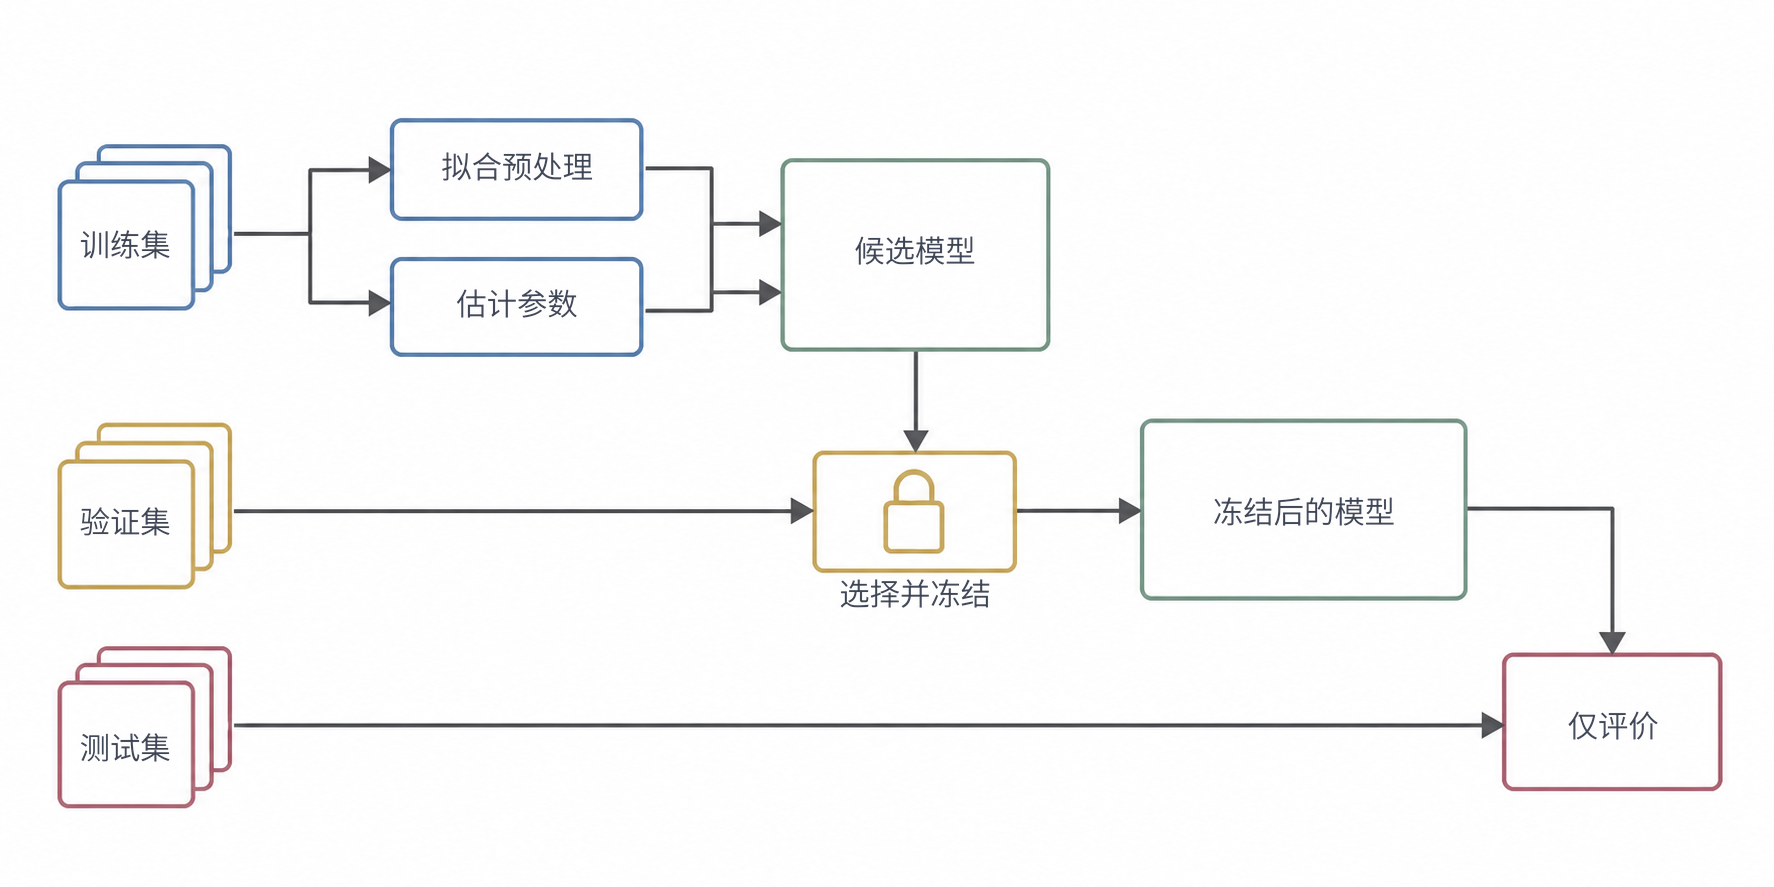
\includegraphics[width=164.600mm]{figures/02-foundations/01-basics/generated/introduction-data-split/figure.png}
  \caption{训练集、验证集和测试集的用途。时间箭头表示一种面向未来预测的划分方式；记录数量仅作示意，不代表划分比例。训练集用于参数学习与预处理拟合，验证集用于配置和停止位置的选择，测试集在这些选择冻结后才用于最终评估。}
  \label{fig:data-split-uses}
\end{figure*}

如果学习或选择过程提前利用了本不应获得的信息，就会发生\term{信息泄漏}
（information leakage）。例如，同一封邮件的副本同时进入训练集和测试集，模型可能靠
记住内容通过测试；先用全体数据选词，再划出测试集，也已经利用了测试数据。
反复查看测试成绩并据此改模型，会使最终模型的选择依赖测试结果；该测试集因此不能再作为
独立于选择过程的最终评价证据。这样的评价往往过于乐观，
因为部署时无法提前利用待预测样本的答案或整批未来数据。

数据划分并不能解决所有问题。一个干净的测试集只能回答“模型在这个测试分布上表现如何”。
如果目标用户、采集设备或时间范围改变，还需要新的验证与监测。数据的来源、生成过程和使用
条件，和数据矩阵本身同样重要。

\section{性能度量}
\label{sec:performance-measures}

性能度量把应用目标变成可比较的数量。选择指标之前，应先说明哪类结果重要、错误代价是否
对称以及与什么基线比较。垃圾邮件系统中，漏放一封广告邮件会打扰用户，误拦一封重要邮件
则可能造成更大损失，因此只报告总体准确率不足以支持部署决策。

要区分两类错误，可以把每封邮件的真实标签和预测标签交叉对照，形成
\term{混淆矩阵}（confusion matrix）：表的四个格子分别记录两种正确判断和两种错误。
在本例中，真正例（true positive, TP）是正确识别
的垃圾邮件，假正例（false positive, FP）是被误拦的正常邮件，假负例（false negative, FN）
是漏放的垃圾邮件，真负例（true negative, TN）是正确放行的正常邮件。
表~\ref{tab:spam-confusion-matrix}由表~\ref{tab:spam-test-results}逐行汇总而来。

\begin{table}[htbp]
  \centering
  \small
  \begin{tabular}{@{}llcc@{}}
    \toprule
    & & \multicolumn{2}{c}{\textbf{预测类别}} \\
    \cmidrule(l){3-4}
    & & 垃圾邮件 & 正常邮件 \\
    \midrule
    \textbf{真实类别} & 垃圾邮件 & TP $=3$ & FN $=0$ \\
                    & 正常邮件 & FP $=2$ & TN $=3$ \\
    \bottomrule
  \end{tabular}
  \caption{垃圾邮件测试结果的混淆矩阵。行表示真实类别，列表示预测类别；
  “垃圾邮件”被约定为正类。}
  \label{tab:spam-confusion-matrix}
\end{table}

我们可以从这张表提出三个不同问题：全部邮件中有多少判对了？拦下的邮件中有多少确实
是垃圾邮件？真正的垃圾邮件又找回了多少？它们分别对应\term{准确率}（accuracy）、
\term{精确率}（precision）和\term{召回率}（recall）。\term{$F_1$值}（F1 score）用
精确率和召回率的调和平均数综合二者，只有二者都较高时才会较高。计算公式为
\begin{align}
  \text{准确率}
    &=\frac{\mathrm{TP}+\mathrm{TN}}
      {\mathrm{TP}+\mathrm{FP}+\mathrm{FN}+\mathrm{TN}},\\
  \text{精确率}
    &=\frac{\mathrm{TP}}{\mathrm{TP}+\mathrm{FP}},\\
  \text{召回率}
    &=\frac{\mathrm{TP}}{\mathrm{TP}+\mathrm{FN}},\\
  F_1
    &=\frac{2\times\text{精确率}\times\text{召回率}}
      {\text{精确率}+\text{召回率}}
      =\frac{2\mathrm{TP}}{2\mathrm{TP}+\mathrm{FP}+\mathrm{FN}}.
  \label{eq:classification-measures}
\end{align}
在本例中，准确率为 $6/8=0.75$，精确率为 $3/5=0.60$，召回率为 $3/3=1.00$，
$F_1=0.75$。召回率为1说明测试集里的垃圾邮件都被识别出来；精确率只有0.60说明被拦截的
5封邮件中有2封其实是正常邮件。使用这些公式时还需检查分母：如果没有邮件被预测为
正类，精确率就不能直接按此计算；如果测试集中没有正类，召回率也同样如此。采用右侧
等价式时，分母为零表示$\mathrm{TP}=\mathrm{FP}=\mathrm{FN}=0$，本书将$F_1$报告为
“不适用”而不任意置零。使用软件工具时也应说明其退化情形约定。

类别极不平衡时，准确率尤其容易掩盖问题。若一万封邮件中只有十封垃圾邮件，全部判为正常
也能得到$99.9\%$准确率，却没有完成识别垃圾邮件的目标。精确率和召回率能从不同角度
揭示这一点，但$F_1$也没有直接表达误拦与漏放的实际代价，不能自动替代应用中的取舍。
提高分类阈值后，被拦截的邮件会减少或保持不变，召回率不会上升；精确率是否提高则取决于
被排除的是正常邮件还是垃圾邮件。阈值应在验证集上根据应用代价选择，不能看过测试结果再调节。

如果预测的是数值，就可以直接检查预测值偏离真实值多远。\term{平均绝对误差}
（mean absolute error, MAE）对偏差的绝对值取平均，\term{均方误差}
（mean squared error, MSE）则对偏差的平方取平均。对$n$个评估样本，记真实值为$y_i$、
预测值为$\hat{y}_i$，则
\begin{align}
  \operatorname{MAE}
    &=\frac{1}{n}\sum_{i=1}^{n}|\hat{y}_i-y_i|,\\
  \operatorname{MSE}
    &=\frac{1}{n}\sum_{i=1}^{n}(\hat{y}_i-y_i)^2.
\end{align}
平方会使大误差受到更重惩罚，因此两者表达不同偏好。排序、生成和序贯决策也各有相应指标，
评价时还可能需要结合人工判断、延迟、资源消耗和长期影响。本章不逐一罗列，而强调指标必须
与任务和使用条件相匹配。

这些指标都是在有限样本上计算的，真正关心的却是未来数据上的表现。式~\eqref{eq:binary-cross-entropy}
给出一次预测的损失，式~\eqref{eq:spam-empirical-risk}把它在训练集上取平均，得到经验风险。
若改为按未来数据的概率规律取平均，就得到\term{期望风险}（expected risk，也称population
risk），即模型
在目标分布上的平均损失。记随机输入及其标签为$(\bm{X},Y)$，目标分布为$\mathcal{P}$，则
\begin{equation}
  R(\bm{\theta})
  =\mathbb{E}_{(\bm{X},Y)\sim\mathcal{P}}
  \left[\ell\bigl(f_{\bm{\theta}}(\bm{X}),Y\bigr)\right].
  \label{eq:expected-risk}
\end{equation}
式中的$\mathbb{E}$表示取期望，也就是按各种情形出现的概率对损失加权平均。
目标分布通常未知，因此用独立测试集估计平均损失或任务指标。这个估计只适用于相应的
采样条件，不能保证任意未来环境中的表现。比较模型时，应使用相同的数据划分、可用信息
和评价口径。预处理方案与阈值可用验证集选择，词表、均值等参数仍只用训练集拟合。
报告时应交代选择方式与估计的不确定性。

\section{本章小结}
\label{sec:introduction-summary}

计算机可以用特征保留输入中的可用信息，以模型假设限定候选规律，再利用历史数据选择具体
模型，从而形成处理新输入的规则。检验这种能力，需要在模型和配置固定后，使用未参与学习的
数据并按任务指标评价结果。垃圾邮件案例走完了这条路径，也说明训练成绩不能单独保证规则
适用于未见邮件。本章把泛化变成了可检验的问题，并未证明它在什么条件下必然可靠。

描述一个学习问题，因而既要说清任务、经验和性能度量，也要交代数据与未来场景的关系。
本例的模型比简单基线识别出更多垃圾邮件，同时误拦了正常邮件，这说明“学得更好”
必须结合实际目标判断。数据是否有代表性、信息是否泄漏、指标是否反映错误代价，
都会改变我们对学习结果的解释。可学习性可以在规定假设下证明算法能够达到相应风险标准；
可信性还要检查这些标准是否覆盖实际后果，以及环境、群体、权限或攻击条件变化后系统是否
仍能工作。前者回答“在这个学习问题中能否学到”，后者回答“学到的结果在实际使用中能否
承担要求”。

\paragraph{延伸阅读}

若想追溯“经验为何能够支持新判断”这一问题，可继续阅读D.~Hume对经验与归纳的讨论，以及
J.~De Houwer等人关于学习定义的综述。若想了解机器学习三要素和早期发展，可分别参见
T.~M.~Mitchell的教材、A.~M.~Turing关于学习机器的讨论以及A.~L.~Samuel的跳棋研究。
后续第~\ref{chap:machine-learning-models}章将建立比较模型的几个基本维度，
第~\ref{chap:machine-learning-paradigms}章系统介绍经验与反馈怎样组织成不同的学习范式，
第~\ref{part:learning-theory}部分进一步追问有限数据在什么条件下能够支持泛化，
第~\ref{part:trustworthy-ml}部分则把这种理论保证放回实际使用条件中检验。
